\section{Overview of \name}
\label{sec:overview}

Stripped of its region-specific constructs, the core language of \name
is a familiar subset of \csharp that includes features such as
class-based inheritance, dynamic dispatch, parametric polymorphism,
and lambdas.  We therefore elide a discussion of the core language,
focusing instead on the concepts specific to region-based memory
management in \name.

\subsection{Stack Regions and Outlives Relation}

Simplest of the region-specific constructs in \name is a \C{letregion}
lexical block that creates a new memory region addressable via its
static identifier. The semantics of the \C{letregion} block is similar
to Tofte and Talpin~\cite{ttpopl94}'s \C{letregion} expression; the
newly introduced region is live only inside the block, where its
identifier is in scope for \C{new} expressions to make allocations
inside the region. For example, in the following code, object \C{a} is
allocated in the region with identifier \C{R0} introduced by the
\C{letregion}:
\begin{center}
\begin{codejava}
  letregion R0 {
    Object a = new@R0 Object();
  }
\end{codejava}
\end{center}
The \C{letregion} blocks can be nested, leading to a stack of regions
that are deallocated in the reverse order in which they are allocated.
Following ~\cite{cyclonepldi02}, we therefore call regions introduced
by \C{letregion} expressions as \emph{stack regions}. The stack
discipline induces an \emph{outlives} relationship among regions created
by nested \C{letregion}s, where the region introduced by the outer
\C{letregion} is guaranteed to outlive the one introduced by the inner
\C{letregion}. It is therefore safe to refer to an object allocated in
outer region from the inner region, but the converse is not true. For
example, consider the following code (assume that class \C{A} has
field \C{x} of type \C{Object}):
\begin{center}
\begin{codejava}
  letregion R0 {
    A a0 = new@R0 A();
    letregion R1 {
      A a1 = new@R1 A();
      a1.x = new@R0 Object(); // safe & legal
      a0.x = new@R1 Object(); // unsafe & illegal
      ...
    }
    ...
  }
\end{codejava}
\end{center}
The code creates two stack regions with identifiers \C{R0} and \C{R1},
where the region \C{R0} outlives the region \C{R1} (denoted as $\C{R0}
\outlives \C{R1}$).  Objects \C{a0} and \C{a1} are allocated in regions
\C{R0} and \C{R1}, respectively. The first assignment statement
assigns to \C{a1.x} an object allocated in outer region (\C{R0}). This
assignment is safe as \C{a1.x} refers to a longer living object, hence
is guaranteed to be a valid reference throughout the lifetime of
\C{a1}.  In contrast, the second assignment is unsafe, as it assigns
to \C{a0.x} an object, whose lifetime is shorter than the lifetime of
\C{a0}, making it unsafe to dereference \C{a0.x} outside the inner
block. 
% Unsafe assignments can also happen indirectly via a function call..
Preempting such unsafe assignments is the \emph{raison d'etre} of the
region type system.

\paragraph{A Note on region identifiers} Every stack region in \name
is associated with a static identifier that uniquely identifies the
region within its scope. At runtime, if a \C{letregion} expression is
evaluated multiple times in a loop or a recursive method, the
corresponding identifier is bound to a new stack region each time. 
Any proposition involving static region identifiers is
considered true at a program location if and only if the proposition
is true under all possible evaluation contexts of that program
location. For instance, consider the following example:
%\begin{minipage}{1.55in}
\begin{numcodejava}
for (int i=0; i<=10; i++) {
  letregion R0 {
    letregion R1 {
      A a1 = new@R1 A();
      ...
    }
  }
}
\end{numcodejava}
%\end{minipage}
%\begin{minipage}{1.4in}
%\begin{codejava}
%void m(int i) {
%  letregion R0 {
%    A a = new@R0 A();
%  }
%  this.m(++i);
%}
%...
%this.m(1);
%\end{codejava}
%\end{minipage}
The identifiers \C{R0} and \C{R1} are bound to new stack regions each
time the loop is evaluated. Nonetheless, the propositions (a). $\C{R0}
\outlives \C{R1}$, and (b). $\C{a1}:\C{A@R1}$ (read as \emph{\C{a1}
refers to an object of type \C{A} contained in region \C{R1}}) are
true at line 5, as they are true under all possible bindings of \C{R0}
and \C{R1} at line 5.

% Interestingly, it is possible for multiple stack regions introduced by
% evaluating a the same \C{letregion} expression to be in outlives
% relationship. For instance, in the following example:
% \begin{codejava}
% void m(A a) {
%   letregion R0 {
%     B b = new@R0 B();
%     b.x = a;
%     this.m(new@R0 A());
%   }
% }
% \end{codejava}
% Stack regions identified by \C{R0} introduced in successive recursive
% calls are in outlives relationship. Consequently, the assignment to
% \C{b.x} should be considered safe. Region type system has to allow for
% this possibility.

\subsection{Allocation Context and Qualified Region Polymorphism}
\label{sec:alloc-ctxt}

As the preceding examples illustrate, the suffix \C{@R} in
\C{new@R} indicates that the newly created object should be allocated in the region labeled \C{R}.
However, \name does not require the allocation region to be specified following a \C{new}.
This is critical, as it enables \name applications to use existing region-oblivious C\# libraries.
In the
absence of explicit specification, \name allocates the newly created
object in its \emph{allocation context}, which is the region at the
top of the stack when \C{new} is executed. For instance, the
\C{findMin} function shown below, which makes explicit use of regions,
calls the standard \C{List} library's \C{listIterator} method:
\begin{center}
\begin{codejava}
  int findMin(List<int> l) {
    assert(!l.isEmpty());
    int min = l.get(0);
    letregion R0 {
      ListIterator<int> iter = l.listIterator();
      while(iter.hasNext()) {
        int n = iter.getNext();
        if (n<min) min = n;
      }
    }
    return min;
  }
\end{codejava}
\end{center}
The \C{listIterator} method neither creates new regions, nor does it
annotate \C{new} expressions with region specifications. Consequently,
all new objects created by the method are allocated in the allocation
context for the call to \C{listIterator}, which in this case is
\C{R0}. 

Observe that \C{listIterator} can be called under multiple different
allocation contexts, and each time it returns a \C{ListIterator}
allocated in its allocation context. The iterator object might hold
references to the list, requiring the list to be allocated in a region
that outlives \C{listIterator}\!'s allocation context. However, modulo
this constraint, \C{listIterator} is not concerned about where the
list is allocated. As such, \C{listIterator} is
\emph{region-polymorphic} with respect to (a). its allocation context
argument, and (b). the allocation region of the list, subject to the
constraint that the later outlives the former. We call such region
polymorphism with constraints in \name as \emph{qualified region
polymorphism}. The provision to elide allocation region
specifications, and the ability to infer qualified region-region
polymorphic types are pivotal to interface region-oblivious standard
library code with region-aware application code in \name. 

%\subsection{Boxed and Unboxed Values}
%
%In \name, like in \csharp, values of some primitive types, such as
%integers and bools, are unboxed, whereas others, such as strings are
%arrays, are boxed. Unlike unboxed values, boxed values are objects,
%hence passed by reference. It is therefore important to be mindful
%of allocation regions for strings and arrays, but not so much for
%integers and bools. For instance, in the following code, the
%assignment to integer variable \C{x} is safe, but the assignment to
%the string variable \C{y} is unsafe, as the allocation region (\C{R0})
%of the string constant has lesser lifetime than \C{y}.
%\begin{center}
%\begin{codejava}
%  int x;
%  string y;
%  letregion R0 {
%    x = 2;
%    y = "Hello, World!";
%  }
%  ...
%\end{codejava}
%\end{center}
%Accordingly, \name's region type system lets the former assignment
%pass by, but flags the later as an error.

\subsection{Dynamic (Transferable) Regions}

\name's stack regions have lexically scoped lifetimes, hence are not
suitable for applications that need to transfer data between
autonomous entities, such as \naiad dataflow operators. To support
these applications, it is imperative to support regions whose
lifetimes transcend the boundaries of lexical blocks, functions, or
even programs. Regions that fit this description in \name are called
\emph{dynamic regions}, or \emph{transferable regions}. 

Transferable regions, like stack regions, are memory regions, but
unlike stack regions, they are first class values of \name; they are
considered objects of \C{Region} class, and, like objects of other
classes, they are created using the \C{new} keyword, can be passed as
arguments, stored in data structures, and returned from methods. Like
a stack region, a transferable region facilitates arbitrary object
allocations, but unlike a stack region, it has a well-defined
\emph{root} object denoting the root of the data structure being
transferred. In a typical dataflow computation, an upstream actor
(e.g., a \C{SELECT} operator) constructs a transferable region, sets
its root to the data structure containing intermediate results, and
then transfers it to a downstream actor (e.g., a \C{COUNT} operator),
which performs further processing. Since a transferable region escapes
the lifetime of the sender, there must be no references from inside of
the transferable region to objects allocated in other memory regions
of the sender. Such references, if exist, may become invalid
references in the context of recipient's address space, jeopardizing
memory safety. \name relies on its region type system to prevent such
unsafe references from being created.

\begin{figure}
\begin{codejava}
  public class Region<T> {
    public Region(Func<void,T> mkRoot);
    public void free();
    public void transfer();
  }
\end{codejava}
\caption{The type signature of the \C{Region} class}
\label{fig:region-class}
\end{figure}
The type signature of \C{Region} class is described in
Fig.~\ref{fig:region-class}. The class is parametric over the type of
the root object (i.e., the \emph{root type}) of the transferable
region it creates. The \C{Region} constructor expects a \C{Func}
object - a higher-order function argument that returns an object of
root type.  The idea is to execute this function with the newly
created transferable region as its allocation context. The object thus
created inside the transferable region will serve as its root object.
For instance, the following code creates a transferable region
(\C{rgn}) and sets its root to the string object returned by its
\C{Func} argument (a lambda expression):
\begin{codejava}
  Region<string> rgn = new Region<string>
                        (() => "Hello");
\end{codejava}
Among the methods of the \C{Region} class, \C{free} deallocates
region's memory, while \C{transfer} transfers the region to a
downstream actor as determined by the run-time. The precise semantics
of \C{transfer} are unimportant in the context of the region type
system; it suffices to understand \C{transfer} as an alias of
\C{free}.

\name imposes a simple discipline on how $\RgnZ$ objects can be used
to perform operations on transferable regions. This discipline is
imposed in the interest of memory safety, which is discussed in the
following subsection.

\subsection{Memory Safety}
\label{sec:memory-safety}

The key to memory safety in \name is the following restriction:
an object $o_1$ in a region $R_1$ is allowed to store a pointer to
an object $o_2$ in a region $R_2$ only if $R_2$ is guaranteed to outlive $R_1$.
(A similar restriction applies in the case where $o_1$ is a stack-allocated variable.)

Enforcing this restriction is simple in the case of stack regions since the outlives relation
between stack regions can be inferred from their lexical nesting. Unfortunately,
inferring outlives relations between transferable regions is not easy.
\name imposes the following protocol on the use of transferable regions to help simplify
this check.

A transferable region (that has not been freed or transferred) can be in one of two possible
states, \emph{open} or \emph{closed}. A newly created region is in the closed state.
A region must be opened, using the open construct (explained in detail below), in order
to read or update or allocate an object within that region.
An open region cannot be freed or transferred. 
In particular, an open region is guaranteed to be live for the entire duration of the open construct.
This allows the type system to infer a valid outlives relation between the opened region
and any stack region that is nested within the open construct.

%Memory safety in \name is primarily due to its region type system,
%although few runtime checks are needed.
%% However, the type system does not ensure the integrity of a small
%% subset of pointers, called the \emph{unsafe set}, for which runtime
%% verification is needed to guarantee safety. This is more a design
%% decision rather than an unfortunate inevitability, as the following
%% discussion elaborates.
%At a fundamental level, the region type system's approach to memory
%safety involves approximating (a). the set of memory regions that are
%live at any given program location\footnote{We say the type system
%tracks \emph{liveness} of memory regions}, and (b).  \emph{outlives}
%relationships between them, and using this information to preempt
%potentially unsafe references from being created. These include:
%\begin{itemize}
%\item References into dead/non-existing regions,
%\item References from longer-living stack regions to shorter-living ones, and 
%\item References that escape transferable regions.
%\end{itemize}
%Maintaining precise approximation of liveness and outlives information
%for stack regions is easy. However, for dynamic (transferable) regions,
%statically determining liveness is equivalent to determining if a C
%pointer is null in presence of dynamic memory allocation, which is
%undecidable in general. Systems that attempt to ensure full memory
%safety in presence of dynamic memory (e.g., ~\cite{henglein},
%~\cite{rust}) do so by conservatively approximating liveness
%information for memory (regions). Maintaining a good conservative
%approximation requires them to employ techniques such as linear
%types~\cite{wadlerlt} or unique pointers~\cite{rust}, which impose
%restrictions that are often too hard to program
%around\footnote{Internet has many tutorials on how to \emph{fight} the
%borrow checker in Rust.}. This is particularly unacceptable in the
%context of \name, as dataflow programs are often run offline, and the
%concern for performance and developer productivity outweighs the
%concern for safety. 
%
%\name's region type system therefore adopts the novel approach of
%overapproximating liveness information for transferable regions, i.e.,
%it might assume that a transferable region is live when, in fact, it
%might have already been transferred or freed. This imprecision should
%be a cause of concern as it can lead to cases where creation of unsafe
%references, and their subsquent dereferencing go unnoticed by the type
%system. Considering that stack regions can contain pointers into
%transferable regions, the worst case cost of overapproximating
%liveness is therefore the integrity of \emph{every} pointer on stack.

%Fortunately, \name avoids this worst case scenario.  \name achieves
%this by imposing a simple state transition discipline on the lifetime
%of a transferable region.  The relevant finite state machine is shown
%in Fig.~\ref{fig:region-fsm}.

The protocol for transferable regions is presented as a finite state machine in Fig.~\ref{fig:region-fsm}.

\begin{figure}
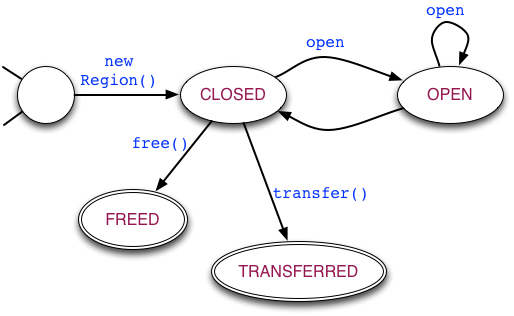
\includegraphics[scale=0.45]{region-fsm.png}
\caption{The lifetime of a dynamic (transferable) region in \name}
\label{fig:region-fsm}
\end{figure}

A transferable region starts its lifetime in a \emph{closed} state,
when it is created through \C{new Region} expression. \name provides
\C{open} lexical construct to \emph{open} a transferable region as an
allocation context, and to access its root object:
\begin{codejava}
  Region<string> rgn = new Region<List<String>>
                        (() => new List<String>());
  open rgn as  strList@R0 {
    strList.addAtHead("World");
    strList.addAtHead("Hello");
  }
  rgn.transfer();
\end{codejava}
In the above code, the \C{open} lexical block performs the
following operations: (a). It opens the transferable region handled by
\C{rgn} for allocation (i.e., makes it the current allocation
context), (b). assigns the identifier \C{R0} to the open region, and
(c). sets the newly introduced local variable (\C{strList}) to refer
to its root object (a list of strings). As Fig.~\ref{fig:region-fsm}
indicates, it is not possible to open a region that is already
transferred/freed. The fact that \C{rgn} is open within the block
therefore guarantees that it is not yet transferred/freed, and that
dereferencing \C{strList} within the block is safe. The end of
\C{open} block marks the return of transferable region to the closed
state.  While closed, the region is eligible to be transferred to a
downstream actor, or to be freed.  An actor that receives the
transferable region, receives it in the closed state. It can then
reopen the received region to read its contents, possibly add more
data and transfer it to another actor, or free the region. 

\name lets stack regions to be used as working memory while operating
with the data stored in a transferable region. Consider the following
code, for instance\footnote{For brevity, we drop the region identifier binding part of the
\C{open} expression whenever the identifier is not used.}:
\begin{codejava}
void onReceive(Region<List<String>> rgn)
  open rgn as strList {
    letregion R1 {
      String s = "";
      ListIterator<String> i = strList.listIterator();
      while(i.hasNext()) {
        s += i.getNext();
      }
      print s; //prints "HelloWorld"
    }
  }
  rgn.free();
}
\end{codejava}
The stack region \C{R1} is being used in the above code to provide
working memory to work with the objects of transferable region
\C{rgn}. Since a transferable region cannot be transferred/freed while
it is still open (Fig~\ref{fig:region-fsm}), \C{rgn} is guaranteed to
outlive the stack region \C{R1} in the above code, making it safe for
the later to contain references to the former. \name therefore allows
such references.

% The design decisions reflected above, \emph{viz.}, to ascribe a root
% object to every transferable region, to make use of a higher-order
% argument to initialize the root object, and to require that a region
% be explictly opened in a lexical block for allocations, were made to
% reflect the message semantics of transferable regions, to promote
% uniform style of programming with different kinds of regions, and to
% precisely state and enforce the safety guarantees offered by \name's
% region type system (\S~\ref{sec:type-system}).

As evident in the above examples, the safety of memory accesses in
\name is now subject to the condition that every transferable region
correctly follows the state transition discipline shown
in Fig.~\ref{fig:region-fsm}. If this is
guaranteed, then \name's region type system statically guarantees the
safety of all memory accesses. In other words, the type system reduces
the problem of ensuring memory safety in \name programs to the problem
of enforcing the state transition discipline for transferable regions.

In \name, this enforcement is done at runtime by explicitly keeping
track of the \emph{current state} for $\RgnZ$ objects, and
checking the validity of every open, transfer, or free operation
and throwing an exception if it is invalid.
The challenge in enforcing this discipline statically is that transferable regions
are first-class objects. Hence, the program can create multiple aliases for
the same region, \eg, open it via one alias and free it via another.
Typestate verification in the presence of aliases is hard.
The checking can be done statically by preventing the creation of aliases using, \eg, linear types
or unique types. However, this would be quite restrictive, in terms of expressiveness.

\name chooses a reasonable trade-off. Regions are coarse-grained objects, manipulated relatively infrequently,
in comparison to manipulations of the fine-grained objects that reside inside regions. Hence, the programmer burden
as well as the runtime overhead of checking the region's state transition discipline is acceptable.

\begin{figure}[t!]
\begin{numcodejava}
class SelectVertex<TIn, TOut> {
  Func<TIn, TOut> selector;
  Dictionary<Time, Region<List<TOut>>> map;
  ...
  void onReceive(Time t,Region<List<TIn>> inRgn){
    if (!map.ContainsKey(t))
       map[t] = new Region<List<TOut>> (
                  () => new List<TOut>());
    open inRgn as inputList {
      letregion R0 {
        foreach (TIn input in inputList) {
          open map[t] as outRgn {
            TOut output = selector(input);
            outRgn.add(output); } } } }
    inRgn.free();
  }
  void onNotify(Time t) {
     Region<List<TOut>> outRgn = map[t];
     map.Remove(t);
     outRgn.transfer();
  }
}
\end{numcodejava}
\caption{\C{SELECT} dataflow operator in \name}
\label{fig:motivating-eg-in-broom}
\vspace*{-0.15in}
\end{figure}


\subsection{An Example}

Fig~\ref{fig:motivating-eg-in-broom} shows how the motivating example
of Fig.~\ref{fig:motivating-eg} can be written in \name.
The \C{onReceive} method receives its input message in a \emph{transferred}
region (\ie, a \emph{closed} region whose ownership is transferred to the
recipient).
Line 7 creates a new region to store the output for time \C{t},
initializing it to contain an empty list.
Line 9 opens the input region to process it.
Line 10 creates a stack region \C{R0}.
Thus, the temporary objects created by the iteration in line 11,
for example, will be allocated in this stack region that lives just
long enough.
We open the desired output region in line 12, so that the new output
objects created by the invocation of \C{selector} in line 13
are allocated in the output region.
Finally, the input region is freed in line 19.

Note that this approach works correctly only if \C{selector}
creates an output object that does not share any subobjects with its input
object (which resides in the input region and will be freed at the end of
the method).
If desired, such subobjects must be cloned (to copy them from the input
region to the output region).
Fortunately, \name's region type system (\S~\ref{sec:type-system}) is
capable of capturing such nuances in the type of \C{selector}
and the type checker will ensure correctness.
Furthermore, the type can be automatically inferred by \name's region type
inference (\S~\ref{sec:type-inference}), which can perform the above
non-trivial reasoning on behalf of the programmer.
